\section{Accessing the data}
Optimization has also a \textbf{hardware} component: accessing the data has to be done efficiently, measuring and modeling physical costs. 

\begin{wrapfigure}{L}{0.5\textwidth}
	\vspace{-15pt}
	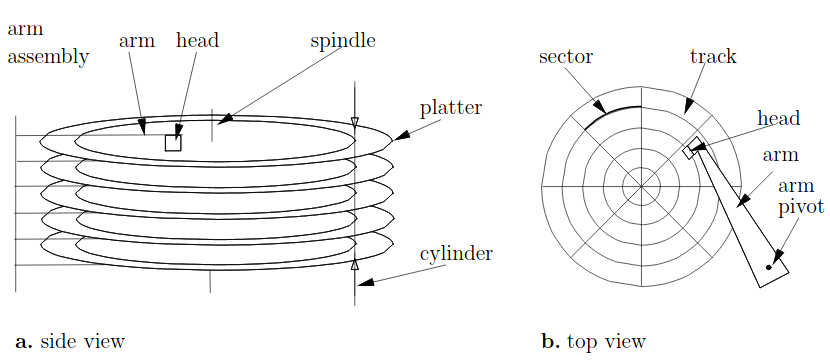
\includegraphics[width=0.5\textwidth]{disk.png}
	\vspace{-25pt}
\end{wrapfigure}

Older devices store memory in a stack of \textit{rotating disks} on which an arm writes data with its head. Each disk is divided in \textbf{tracks} and \textbf{sectors}, of which the outer are longer than the inner.

Cylinders are organized in zones: each of them contains a fixed number of consecutive cylinders, with the same amount of sectors per track. 

Since the disk is rotating, the throughput is higher on outer cylinders, and reading is only possible where the head is, making this operation quite slow since it is impossible to jump. On SSD, this is indeed implemented.

A good approximation of the \textbf{seek time} among $d$ cylinders is:
$$seektime(d) = \begin{cases}
	c_1 + c_2\sqrt{d} & d \leq c_0 \\
	c_3 + c_4d & d> c_0
\end{cases}$$
Constants indicate the maximum number of cylinders where no coast take place, i. e. the point in which the head can be efficient. 

The square is introduced because in the low part of hardware the distance is less, hence the head moves faster. On the other hand, the formula is linear if the distance is short.

Since the current position on the disk is unpredictable, it is difficult to produce single cot estimation, however modeling many accesses gives a somewhat accurate measurement. 

\begin{wrapfigure}{R}{0.5\textwidth}
	\vspace{-15pt}
	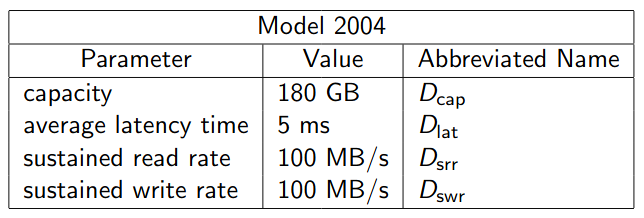
\includegraphics[width=0.5\textwidth]{parameters.png}
	\vspace{-30pt}
\end{wrapfigure}

Parameters are aggregated, introducing average latency time (for positioning) and sustained read/write assuming a sequential scan. 

The time a disk needs to read and transfer $n$ bytes is approximately $D_{lat} + \frac{n}{D_{srr}}$. Examples of these values are given in the table.

Database developers, as introduced before, distinguish between \textbf{random} and \textbf{sequential} access. The latter is faster, since it assumes data only needs to be \textit{read in sequence} after finding its position, while a random access implies seeking the location of each page (the smallest portion which can be read, generally 8kb).

Example: to read 100MB, sequential read takes $5ms + 1ms$, while random read has to scan 8k pages and takes $65s$.

This has consequences in practice: for instance, an index may be efficient only if a \textit{small portion of the data is accessed}, else there is a risk for the whole structure to be traversed with a random access behavior. On the other hand, it could be expensive to perform a scan if there are many pages involved. 

\subsection{Counting the number of accesses}
A proposed cost function to calculate sequential scan time is: 
$$5ms + \frac{\abs{page\_size}}{\abs{bandwidth}} * \#pages$$
Now, the problem becomes estimating the bandwidth, the number of needed pages and their cost. These can vary between different use cases, or be influenced by indexes. 

More parameters are introduced for a better overview, assuming a uniform distribution of the tuples:
\begin{itemize}
	\item $N$, number of tuples (items) in relation $R$;
	\item $m$, number of pages (buckets) in which tuples of $R$ are stored ($m = 1$ all pages are accessed);
	\item $B = \frac{N}{m}$, tuples for page (blocking factor);
	\item $k$, number of distinct TID ($k = 1$ implies one page is accessed).
\end{itemize}
The probability to request a set with $k$ items is $\frac{1}{{{N}\choose{k}}}$, because of the uniformity assumption.

\subsubsection{Yao's formula (direct, uniform, distinct)}
Considering $m$ buckets with $n$ items, then there is a total of $N = nm$ items. Randomly selecting $k$ \textbf{distinct} items give a number of qualifying buckets which is:

$$\bar{y}^{N, m}_n(k) = m * y^N_n(k)$$
$$y^N_n(k) = \begin{cases}
	[1 - p] & k \leq N - n \\
	1 & k > N - n
\end{cases}$$
$y^N_n(k)$ is the probability that bucket $n$ contains at least one tuple, and $p$ is the probability that a bucket contains none of the $k$ items.
\begin{wrapfigure}{R}{0.25\textwidth}
	\vspace{-25pt}
	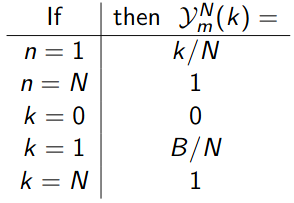
\includegraphics[width=0.25\textwidth]{yao.png}
	\vspace{-30pt}
\end{wrapfigure}
$$p \quad = \quad \frac{{{N-n}\choose{k}}}{{{N}\choose{k}}} \quad = \quad \prod_{i=0}^{k-1} \frac{N-n-i}{N-i} \quad = \quad \prod_{i=0}^{n-1}\frac{N-k-i}{N-i}$$
These formulas are useful to avoid computing $N!$, which is too expensive to do in practice. The choice of formula depends on $N$ and $k$.

However, even with simplifications, calculations are not cheap, and fractions may not be integers: further steps must be taken, such as introduction of a Gamma function and approximations (\textbf{Waters}):
$$p \approx \Big( 1 - \frac{k}{N} \Big)^n$$
This works implying there is a fraction of $\frac{k}{N}$ tuples which are relevant for the query, multiplied for the number of pages. The problem here is, if the first tuple does not qualify, the likelihood that a latter one qualifies increases (there is less space); in general, probability is not uniform.

The estimation is roughly accurate with $N >> n$, and much cheaper to compute. There are other formulas which are simpler, but more complicated to express (\textbf{Bernstein}):
$$y_n^{N,m}(k) \approx \begin{cases}
	k & k < \frac{m}{2} \\
	\frac{k+m}{3} & \frac{m}{2} \leq k \leq 2m \\
	m & 2m \leq k
\end{cases}$$
This evaluation tries to interpolate $k$ depending on its comparison with $m$, and is faster to compute. Each case is plausible, yet not very precise. 

Dihr and Saharia computed some upper and lower bounds for $p$, claiming these are accurate with a minimal difference from real-case scenarios.

\subsubsection{Cheung's formula (direct, uniform, non-distinct)}
Index nested loop joins often involve reading the same tuple multiple times, fetching join partners using the index. This strategy uses very little memory, with time linear in the left side.

In this case, Yao's formula is not sufficient, and a \textbf{multiset} (set with duplicates) approach is introduced. The number of multiset with cardinality $k$ containing only elements from a set $S$ with $\abs{S} = N$ is:
$${N+k-1}\choose{k}$$

This works transforming a multiset into a set by summing a crescent value from 1 to $(k-1)$ to each element, making them unique. The other way around applies subtraction. 

Cheung's formula is an extension of Yao's formula considering multisets (not necessarily distinct items among $k$):
$$\overline{Cheung}^{N, m}_n(k) = m * Cheung^N_n \qquad Cheung^N_n(k) = [1 - \tilde{p}] \qquad \tilde{p} \approx \Big( 1 - \frac{n}{N}\Big)^k$$
$$\tilde{p} \quad = \quad \frac{{n-n+k-1\choose k}}{{n+k-1\choose k}} \quad = \quad \prod_{i=0}^{k-1} \frac{N-n+i}{N+i} \quad = \quad \prod_{i=0}^{n-1} \frac{N-1-i}{N-1+k-i}$$
This just expands binomials using the duplicates property. The approximation of $p$ (\textbf{Cardenas}) is derived assuming there are $1 - \frac{n}{N}$ tuples on the current page and applying the power.

The number of \textbf{distinct} values in a $k$-multiset of cardinality $N$ with uniform distribution is:
$$D(n, k) = \frac{Nk}{N + k - 1}$$
This follows by previous statements, expanding the binomial coefficient. This allows to do a simplification (\textit{model switching}), i. e. using Yao's formula after removing duplicates. 

Non-uniform distributions work similarly, yet modeling each probability to access a group of buckets, using summation instead of product. 

\subsection{Sequential accesses on disk}
Accesses on disk are relevant to estimate the cost of \textbf{jumping between two pages or cylinders}: this directly depends on the distance gap. When estimating seek costs, there must be a probability distribution for the distances.  

Assuming the situation is a \textbf{bitvector} of length $B$ with $b$ bits set to 1, then $B - b$ bits are zero, and the accesses can be modeled with $B$ corresponding to the number of cylinders while $b$ indicates that a cylinder qualifies.

Then, the probability distribution of the number $j$ of zeros between two consecutive ones, before the first or after the last is:
$$B^B_b(j) = \frac{{B-j-1\choose b-1}}{{B\choose b}} = \frac{b}{B-j}\prod_{i=0}^{j-1} \Big( 1 - \frac{b}{B - i}\Big)$$
The distance between two ones is obtained taking the expected value of the number of zeros, and adding one for the potential first or last position.

Some other values can be deduced from this, such as the total number of bits from the first bit to the last one (extremes included), which is:
$$B_{tot}(B, b) = \frac{Bb + b}{b + 1}$$
All these computations have several real-life applications: the original motivation implies retrieving values from a B-tree and accessing them on disk, sorting the entries to avoid multiple random lookups. A bitvector module gives information about the distance between pages, to understand how expensive a fetch can be.

\section{Selectivity estimations}
Selectivity estimation has always been assumed to be known until now, yet it is a statistic which needs to be computed, since it is essential for query optimization.

Unfortunately, this is a \textit{fundamentally difficult problem}, and can take quite a long time.

Specifically, there are different selectivity problems requiring different approaches. For arbitrarily difficult queries it is impossible to make an estimation, yet the following three are the most common:

\begin{lstlisting}[language=SQL]
SELECT *
FROM relation r
WHERE r.a = 10
	
SELECT *
FROM relation r
WHERE r.b > 2
	
SELECT *
FROM relation1 r1, relation2 r2
WHERE r1.a = r2.b
\end{lstlisting}

\subsection{Heuristic estimations}
There are some textbook estimations which are not advanced strategies, depending on the predicate.

\begin{wrapfigure}{R}{0.6\textwidth}
	\vspace{-20pt}
	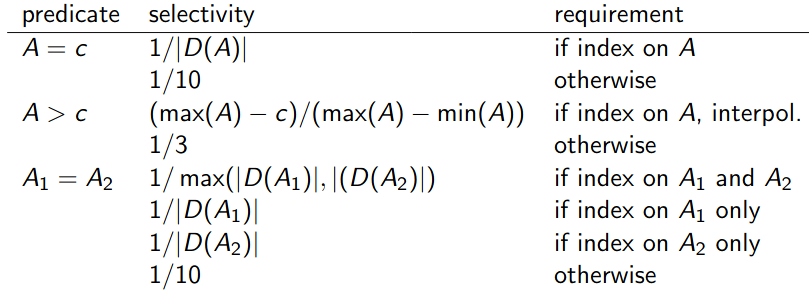
\includegraphics[width=0.6\textwidth]{selectivity.png}
	\vspace{-30pt}
\end{wrapfigure}

Knowing the domain of $A$, for instance, can happen when the column has an \textbf{index}, yet an uniform distribution must be assumed.

Having a range query is also helped by an index, since this additional data structure stores the minimum and maximum value, hence selection can be obtained by interpolation. 

Joins again depend on indices and domain of the involved tables.

\subsection{Building histograms}
Heuristics are quite simple and have the restriction of uniform distribution, so multiple DBMS employ histograms: aggregated data is \textbf{partitioned in buckets} such that $H_A(b) = |\{r\ |\ r \in R \;and R.A \in b\}|$ and thus $\sum_{b \in B} H_A(b) = \abs{R}$.

This methods leads to a much better estimation than previous ones, and computing histograms is also easy since it only involves a sequential scan: the real challenge is selecting the appropriate $B$.

Assuming data is already in buckets, there are formulas giving the appropriate result, applying linear interpolation to the newly obtained histogram:
$$A = c \quad \frac{\sum_{b \in B:c \in b H_A(b)}}{\sum_{b \in B}H_A(b)}$$
$$A > c \quad \frac{\sum_{b \in B:c \in b \frac{max(b) - c}{max(b) - min(b)} H_A(b) + \sum_{b \in B:min(b) > c} H_A(b)}}{\sum_{b \in B}H_A(b)}$$
$$A_1 = A_2 \quad \frac{\sum_{b_1 \in B_1, b_2 \in B_2, b' = b_1 \cap b_2: b' \neq \emptyset} \frac{max(b') - min(b')}{max(b_1) - min(b_1)} H_{A_1}(b_1) \frac{max(b') - min(b')}{max(b_2) - min(b_2)} H_{A_2}(b_2)}{\sum_{b_1 \in B_1}H_{A_1}(b_1) \sum_{b_2 \in B_2}H_{A_2}(b_2)}$$

These computations only give an upper bound, while the lower bound can be up to zero, and it is impossible to predict. Furthermore, the upper bound can be quite an overestimation in the first case, which represents only a rough approximation.

The problem comes from the restriction in the mathematical meaning of $P(A = c) = 0$, which gives a sound result when $A > c$ but fails when the query involves equality. Joining works using some assumptions as well, such as independence.

\subsubsection{Equiwidth}
Building histograms concerns the previously mentioned issue: finding the optimal number of buckets. Typically, this is a fixed value, and it has to work with an unknown distribution.

One particular strategy is partitioning the domain into buckets of equal width, simply constructing them from left to right. This is easy to compute, since it does not require boundaries: it is enough to store minimum, maximum and size. 

However, it fails when data is skewed, causing uneven buckets and therefore a greater estimation error. 

\subsubsection{Equidepth}
Another method is the equidepth, forcing each bucket to have the same number of elements, adopting to data distribution. This technique is very common and not too time consuming, so it is widely used in practice.

The only disadvantages are having to sort the values beforehand, and store boundaries and ties (obviously not the count).

\subsubsection{Interpolation}
Interpolation is a technique to improve accuracy, however it can be difficult to interpolate a histogram: a potential solution is using the distribution function instead, which is continuous and monotonic. This works particularly well in the case $A > c$.

Further research includes analyzing correlations, multi-dimensional histograms and cardinality estimators.